\documentclass[conference]{IEEEtran}
\usepackage{graphicx}
\usepackage{booktabs}
\usepackage{url}
\usepackage{amsmath}
\usepackage[hidelinks]{hyperref}
\usepackage{balance}

\begin{document}

\title{How Well Does AI Understand Nepali?\\
A Multi-Task Benchmark of Large Language Models and Embedding Models on a Low-Resource Language}

\author{\IEEEauthorblockN{Ramesh Kadariya}
\IEEEauthorblockA{ISMT College (University of Sunderland)\\
Chitwan, Nepal\\
Email: contact@rameshkadariya.com.np\\
Web: \url{https://rameshkadariya.com.np}}}

\maketitle

\begin{abstract}
Modern language models are trained predominantly on English, yet they are increasingly deployed to speakers of low-resource languages. This paper presents a reproducible multi-task benchmark measuring how well current large language models (LLMs) and text embedding models handle Nepali, a Devanagari-script language spoken by more than 30 million people. Five tasks are evaluated: tokenizer fertility, paired reading comprehension, sentiment classification of native social media text, machine translation in both directions, and embedding-based passage retrieval. All evaluation data derives from openly licensed sources, all sampling is fixed by seed, and every reported number is generated by published scripts from published raw model outputs. Four main findings emerge. First, tokenization imposes a direct cost penalty on Nepali users: on identical parallel content, the GPT-4 era cl100k tokenizer consumes 4.79 times more tokens for Nepali than for English, and popular open-model tokenizers consume 2.1 to 4.5 times more, whereas multilingual-first tokenizers approach parity, showing the penalty is a design choice rather than a property of the script. Second, comprehension degrades with model scale and recency: on identical Belebele questions, Llama 3.1 8B falls from 84.0\% accuracy in English to 57.0\% in Nepali, while frontier-class models retain most of their ability, with Gemini 3.1 Flash Lite falling only from 97.0\% to 89.5\%; all within-model language gaps are statistically significant under McNemar's exact test. Third, an evaluation-methodology hazard is documented: Llama 3.1 8B answered 71 of 200 Nepali items using Devanagari numerals, which a conventional ASCII answer parser silently scores as failures, understating its accuracy by 16.5 points; low-resource evaluation pipelines must parse answers in the script of the question. Fourth, capability is asymmetric: models translate out of Nepali far better than into it, and even strong models reach only 51.9\% to 67.1\% accuracy on three-class sentiment classification of informal native Nepali text, with the neutral class failing almost completely for most models. On retrieval, modern multilingual embedding models perform well (BGE-M3 reaches 84.0\% Recall@1), showing that Nepali retrieval-augmented generation is already feasible if embedding models are chosen carefully. The complete benchmark, data, code, and raw outputs are available at \url{https://github.com/RameshKadariya/nepali-llm-benchmark}.
\end{abstract}

\begin{IEEEkeywords}
low-resource languages, Nepali, large language models, benchmark, tokenization, multilingual NLP, embeddings, retrieval-augmented generation, evaluation methodology
\end{IEEEkeywords}

\section{Introduction}
Large language models have moved from research artifacts to general-purpose infrastructure. They draft documents, answer questions, translate, tutor, and increasingly mediate access to information itself. Their training data, however, is overwhelmingly English: by most published estimates English constitutes the large majority of web-crawled pretraining corpora, while thousands of languages together share the remainder. The consequences of this imbalance are usually discussed abstractly. This paper measures them concretely for one language.

Nepali (ISO 639-1: \emph{ne}) is the official language of Nepal and is spoken by more than 30 million people in Nepal, India, and a large global diaspora. It is written in the Devanagari script, is morphologically rich, and exhibits pervasive code-mixing with English and Hindi in informal digital communication. Despite its speaker population, Nepali is firmly a low-resource language in the NLP sense: it forms a negligible share of common crawled corpora, has few curated evaluation datasets, is rarely reported in model cards, and until recently had almost no dedicated pretrained models.

The stakes are practical rather than academic. Nepal's public services, education system, and businesses are digitizing rapidly, and AI assistants are already being used by Nepali speakers through the same commercial interfaces that serve English speakers. Two questions therefore matter to millions of users and to anyone building systems for them. First, how much of a model's advertised capability survives when the interaction language is Nepali rather than English? Second, what hidden costs, in money and in usable context window, do Nepali speakers pay when using systems that are billed and bounded per token?

Answering these questions rigorously faces an obstacle that is itself part of the story: evaluation resources for Nepali are scarce, fragmented, and sometimes gated. This work turns that constraint into a design principle. Every dataset used is openly licensed and publicly downloadable; every model evaluated is accessible either locally on commodity hardware or through free API tiers; and the entire experimental pipeline, from dataset freezing to statistical testing to figure generation, is published so that any researcher, including those without institutional funding, can reproduce or extend it. The total inference budget of this study was zero.

\subsection{Research Questions}
The benchmark is organized around five research questions:
\begin{enumerate}
\item \textbf{RQ1 (Cost):} How many more tokens does identical content require in Nepali than in English across current tokenizers, and therefore how much more do Nepali users pay per unit of meaning?
\item \textbf{RQ2 (Comprehension):} When the same reading comprehension questions are posed in English and in Nepali, how much accuracy does each model lose, and is the loss statistically significant?
\item \textbf{RQ3 (Real-world text):} How well do models handle authentic, informal, native Nepali text, as opposed to the formal translated text that dominates multilingual benchmarks?
\item \textbf{RQ4 (Generation):} Is capability symmetric between understanding Nepali and producing it, measured through translation in both directions?
\item \textbf{RQ5 (Retrieval):} Can current embedding models support retrieval-augmented generation (RAG) over Nepali documents, monolingually and cross-lingually?
\end{enumerate}

\subsection{Contributions}
The contributions of this work are:
\begin{enumerate}
\item A frozen, openly licensed, fully reproducible five-task evaluation suite for Nepali covering tokenizer fertility, reading comprehension, sentiment classification, machine translation, and embedding retrieval, with all sampling fixed by random seed and complete provenance documentation.
\item A paired experimental design for comprehension in which the same 200 questions are evaluated in English and Nepali for every model, so that language effects are measured within-model on identical content and tested with McNemar's exact test on paired correctness.
\item Empirical results for six LLMs spanning three orders of magnitude in parameter count (0.5B to 120B plus a frontier commercial model) and six embedding models, all obtained with zero inference budget using single-core CPU inference and free API tiers, demonstrating that rigorous low-resource evaluation is accessible to independent researchers.
\item Quantification of the tokenizer cost penalty for Nepali across twelve tokenizers spanning four generations of design, connecting tokenizer vocabulary construction directly to the price and context capacity experienced by Nepali users.
\item Documentation of a concrete evaluation-methodology hazard for Devanagari-script languages: models may answer multiple-choice questions in Devanagari numerals, which standard ASCII answer parsers silently misscore; correcting this changed one model's measured Nepali accuracy by 16.5 percentage points in this study.
\end{enumerate}

All code, frozen data, raw per-item model outputs, generated tables, and figures are public in the project repository.\footnote{\url{https://github.com/RameshKadariya/nepali-llm-benchmark}}

\section{Related Work}
\subsection{Multilingual Evaluation Benchmarks}
The FLORES family established carefully constructed parallel evaluation for low-resource machine translation: FLORES-101 \cite{goyal2022flores} and its extension to more than 200 languages within the No Language Left Behind project \cite{nllb2022} provide professionally translated parallel sentences spanning diverse domains. Belebele \cite{bandarkar2024belebele} builds multiple-choice reading comprehension on top of FLORES passages in 122 language variants, including Nepali (\texttt{npi\_Deva}), with items aligned across languages. This alignment property is central to the present study: it permits a strictly paired design in which language is the only variable between conditions. Broader multilingual suites such as XTREME and MEGA-style evaluations report aggregate scores over many languages but rarely analyze any single low-resource language in depth; this paper takes the opposite approach, examining one language across many complementary axes.

\subsection{Tokenizer Fairness and the Cost of Language}
Subword tokenizers allocate their fixed vocabulary budget according to the statistics of their training corpus, so languages underrepresented in that corpus fragment into more, shorter tokens. Petrov et al. \cite{petrov2023tokenizers} demonstrated that this induces length differences of up to an order of magnitude between languages and argued the resulting unfairness affects cost, latency, and effective context. Ahia et al. \cite{ahia2023cost} connected fragmentation directly to the money charged by commercial APIs, coining the framing of languages having different prices. This study extends that line to the current generation of tokenizers (o200k, Llama 3, Qwen 2.5, DeepSeek V3, Gemma 2) measured specifically on Nepali parallel text, and adds a Nepali-specific tokenizer (NepBERTa) as an inverted reference point.

\subsection{Multilingual Text Embeddings and Retrieval}
Dense retrieval quality determines the ceiling of RAG systems. Sentence-BERT \cite{reimers2019sbert} popularized sentence-level embedding models; LaBSE \cite{feng2022labse} targeted cross-lingual alignment across 109 languages; multilingual E5 \cite{wang2024e5} applied large-scale contrastive pretraining with instruction prefixes; and BGE-M3 \cite{chen2024bgem3} unified dense, sparse, and multi-vector retrieval across more than 100 languages. Public reporting for these models on Nepali specifically is essentially absent, and practitioner defaults are frequently English-only models such as all-MiniLM-L6-v2. Task 5 quantifies exactly what those choices cost on Nepali content.

\subsection{Nepali Natural Language Processing}
Dedicated Nepali NLP resources remain scarce. NepBERTa \cite{timilsina2022nepberta} pretrained a monolingual BERT on a Nepali corpus and is used here as a tokenizer reference. Public Nepali sentiment corpora exist mainly as social media collections with varying documentation quality; the corpus used here was selected for authenticity of register (native user-generated text rather than translations) and subjected to documented cleaning and native speaker label verification. To the author's knowledge, no prior work has combined cost, comprehension, generation, real-register understanding, and retrieval for Nepali in a single reproducible suite with published raw outputs.

\section{Benchmark Design}
\subsection{Design Principles}
Four principles governed the design. \textbf{Openness}: only openly licensed, ungated data sources are used, so that anyone can rebuild the evaluation sets byte-for-byte. \textbf{Determinism}: all sampling uses a fixed seed (42) and evaluation always reads frozen files, never live sources; a single script (\texttt{src/prepare\_data.py}) constructs every frozen set. \textbf{Pairing}: wherever possible, the identical content is evaluated in both languages so that language is isolated as the experimental variable. \textbf{Transparency of failure}: raw per-item model outputs are published, quota-truncated runs are disclosed with exact sample sizes, and scoring corrections (Section V-C) are documented rather than silently applied.

\subsection{Data Sources and Provenance}
Two openly licensed sources supply all evaluation data. Full construction details are in the repository (\texttt{data/PROVENANCE.md}).

\textbf{Belebele} \cite{bandarkar2024belebele} (CC-BY-SA 4.0). The \texttt{npi\_Deva} and \texttt{eng\_Latn} test splits contain 900 multiple-choice questions each, with four options and one correct answer, aligned across languages by passage link and question number. All 900 Nepali items align exactly with their English counterparts. The passages originate from FLORES-200 and cover news-style and encyclopedic prose. Because FLORES+ and IN22 are gated on the HuggingFace Hub and this benchmark admits only ungated sources, the parallel Nepali-English passage pairs used for the translation and retrieval tasks are extracted from Belebele, which redistributes the FLORES passages openly with cross-language alignment. There are 488 unique parallel passages, typically two to five sentences long; translation is therefore evaluated at passage level.

\textbf{NepaliSentiment} (HuggingFace: \texttt{Shushant/NepaliSentiment}). This corpus contains 6{,}000 items of authentic Nepali user-generated text, primarily comments from stock market forums and video platforms, labeled 0/1/2. The register is genuinely informal: colloquial spellings, romanized fragments, code-mixing, and domain slang all occur. Label semantics are undocumented upstream and were determined by systematic manual inspection of samples from each class, yielding 0 = negative, 1 = positive, 2 = neutral; the mapping was verified by the author, a native Nepali speaker, and a 30-item validation sample ships with the repository for independent review. Cleaning removed rows with malformed labels (8 rows contained values such as dashes or out-of-range numbers), texts shorter than 15 or longer than 500 characters, texts containing fewer than 10 Devanagari characters (removing English-only and emoji-only rows), and exact duplicates. The surviving class pools contain 1{,}299 negative, 1{,}701 positive, and 853 neutral items.

\subsection{Frozen Evaluation Sets}
From these sources the following sets were frozen with seed 42 and are stored as JSONL in \texttt{data/frozen/}:
\begin{itemize}
\item \texttt{qa\_ne.jsonl} / \texttt{qa\_en.jsonl}: 200 paired reading comprehension items per language, sampled from the 900 aligned pairs.
\item \texttt{translation\_pairs.jsonl}: 150 parallel passages sampled from the 488 unique pairs.
\item \texttt{retrieval\_corpus\_ne.jsonl}: all 488 unique Nepali passages.
\item \texttt{retrieval\_queries.jsonl}: 200 queries with known gold passage, one question per unique passage to avoid corpus-frequency bias, each provided in both a Nepali and an English variant.
\item \texttt{sentiment\_ne.jsonl}: 210 items, stratified 70 per class and shuffled.
\item \texttt{validation\_sample.jsonl}: 30 items (15 sentiment, 10 comprehension, 5 translation) for native speaker review.
\end{itemize}

\subsection{Tasks and Metrics}
\textbf{Task 1, tokenizer fertility (RQ1).} Each of twelve tokenizers encodes the 150 parallel passages in both languages. Reported are fertility, defined as tokens per whitespace-delimited word, and the cost ratio, defined as Nepali tokens divided by English tokens for the same passage, averaged over passages. Because commercial APIs bill per token and bound context per token, the cost ratio translates directly into money and usable context.

\textbf{Task 2, reading comprehension (RQ2).} Accuracy on the paired Belebele items. Two protocols are used depending on access mode. API-served chat models answer generatively at temperature 0; the prompt presents the passage, the question, and the four numbered options, and instructs the model to reply with only the number of the correct option, with instructions written in the language under test. The first option numeral in the reply, in either ASCII or Devanagari digits (Section V-C), is the prediction; replies with no parseable option numeral count as incorrect abstentions. The locally run small model is scored by length-normalized log-likelihood over the four options, the standard protocol of the lm-evaluation-harness for Belebele-style tasks, which is deterministic and applicable without instruction following. The within-model language effect is tested with McNemar's exact test on the paired correctness table, using only items completed in both languages.

\textbf{Task 3, sentiment (RQ3).} Three-class classification of the 210 native items. The instruction is written in Nepali and requests a one-word answer; parsing accepts the Nepali label words and their English equivalents. Accuracy, macro-F1, and per-class precision, recall, and F1 are reported. Chance accuracy is 33.3\%.

\textbf{Task 4, translation (RQ4).} Passage-level translation in both directions at temperature 0, with the model instructed to output only the translation. chrF++ \cite{popovic2017chrf} is the primary metric because character n-gram measures are robust for morphologically rich Devanagari text; BLEU \cite{papineni2002bleu} is reported secondarily via sacreBLEU \cite{post2018sacrebleu}, using flores200 sentencepiece tokenization when the output language is Nepali, since word-boundary tokenizers are unreliable for Devanagari.

\textbf{Task 5, retrieval (RQ5).} Each embedding model encodes the 488-passage Nepali corpus and the 200 queries under two settings: monolingual (Nepali query over Nepali corpus) and cross-lingual (English query over Nepali corpus). Similarity is cosine over L2-normalized embeddings; E5 models receive their documented query and passage prefixes. Recall@\{1,5,10\} and MRR@10 are reported. The gold passage for each query is the passage the question was originally written against. An English-only model, all-MiniLM-L6-v2, is included deliberately as a negative control representing a common practitioner default.

\section{Experimental Setup}
\subsection{Models Under Test}
Six LLMs are evaluated, chosen to span three orders of magnitude of scale and both open and commercial access:
\begin{itemize}
\item \textbf{Qwen2.5-0.5B-Instruct} \cite{qwen2025}, run locally in float32 on a single CPU core, representing the smallest class of model deployable offline on inexpensive hardware of the kind realistically available in Nepal.
\item \textbf{Llama 3.1 8B Instruct} and \textbf{Llama 3.3 70B} \cite{grattafiori2024llama}, and \textbf{Llama 4 Scout 17B}, via the Groq free API tier.
\item \textbf{GPT-OSS 120B} \cite{openai2025gptoss}, OpenAI's open-weight model, via the Groq free tier.
\item \textbf{Gemini 3.1 Flash Lite}, a current commercial frontier-family model, via the Google AI Studio free tier.
\end{itemize}
Six embedding models are evaluated locally on CPU: multilingual-e5-small and multilingual-e5-base \cite{wang2024e5}, paraphrase-multilingual-MiniLM-L12-v2, LaBSE \cite{feng2022labse}, BGE-M3 \cite{chen2024bgem3}, and all-MiniLM-L6-v2 as the English-only control. Twelve tokenizers are analyzed, listed in Table \ref{tab:tok}; gated tokenizers were accessed through ungated mirrors where necessary, documented in the code.

\subsection{Inference Protocol}
All generative evaluation uses temperature 0 with a single fixed prompt template per task and language. No few-shot examples, chain-of-thought elicitation, or retry-on-failure heuristics are used; the goal is to measure default behavior under a reasonable direct instruction, not the ceiling achievable by prompt engineering. Local log-likelihood scoring batches the four answer options in one left-padded forward pass, restricted to option-position logits to bound memory; the batched implementation was verified to produce scores identical to sequential scoring. Every API request and every local scoring step appends its raw result to a per-model progress file before proceeding, making all runs resumable and leaving a complete audit trail that is published with the repository.

\subsection{Zero-Budget Constraint and Partial Samples}
The study was executed without paid inference, by design, to demonstrate feasibility for independent researchers in low-resource settings. This constraint has a visible cost that is reported rather than hidden: free API tiers impose per-minute and per-day token quotas, and where a quota was exhausted before a run completed, evaluation stopped at the quota boundary. The affected runs are Llama 3.3 70B comprehension (178 of 200 paired items), GPT-OSS 120B sentiment (158 of 210), Gemini 3.1 Flash Lite sentiment (90 of 210), and the local Qwen2.5-0.5B Nepali comprehension run (37 paired items, bounded by single-core compute time rather than quota). Translation results for GPT-OSS 120B and Gemini 3.1 Flash Lite were excluded entirely because fewer than ten passages completed before quota exhaustion. All partial runs are prefix samples of the same fixed random item order, not selectively chosen subsets, and paired comparisons are always computed on the intersection of completed items. A 21-item English-only probe of the Gemini flagship model, terminated by a 25-request daily quota, is excluded from all tables.

\subsection{Statistical Testing}
For the paired comprehension design, the null hypothesis is that a model is equally likely to flip from correct-in-English to wrong-in-Nepali as the reverse. McNemar's exact test \cite{mcnemar1947} is applied to the discordant pair counts using an exact binomial computation, which remains valid at the small discordant counts observed here. Discordant counts in each direction are reported alongside p-values so readers can inspect the asymmetry directly.

\section{Results}
\subsection{Task 1: The Tokenizer Cost Penalty (RQ1)}
Table \ref{tab:tok} and Fig. \ref{fig:tok} report fertility and cost ratios over the 150 parallel passages; Fig. \ref{fig:fert} visualizes fertility per language. Averaged over the corpus, English fertility is remarkably stable across tokenizers (1.22 to 1.55 tokens per word for all general-purpose designs), while Nepali fertility varies by nearly a factor of six, from 1.73 (BLOOM) to 10.92 (GPT-2). The result is three clearly separated regimes.

\textbf{English-centric designs charge Nepali heavily.} The GPT-4 era cl100k tokenizer needs 4.79 times more tokens for Nepali than English on identical content; Qwen 2.5 (4.46x) and Mistral v0.3 (4.43x) are equivalent. In absolute terms, the 150-passage corpus that costs 14{,}712 cl100k tokens in English costs 70{,}476 tokens in Nepali. A Nepali user of such a system pays nearly five times more money per unit of information and fits nearly five times less material into the same context window, before any quality difference is considered.

\textbf{Partially multilingual vocabularies halve the penalty.} DeepSeek V3 (2.99x), Llama 3.1 (2.60x), and Gemma 2 (2.14x) show what larger, more internationally balanced vocabularies buy.

\textbf{Multilingual-first designs approach parity.} GPT-4o's o200k tokenizer reaches 1.62x, a threefold improvement over its predecessor cl100k within the same product family; mT5 (1.46x), NLLB-200 (1.19x), and BLOOM (1.18x) approach parity. The Nepali-specific NepBERTa inverts the relationship entirely at 0.47x, encoding Nepali more compactly than English.

The cl100k-to-o200k comparison is the cleanest evidence in the study that the Nepali penalty is a vocabulary design decision, not an inherent property of Devanagari: the same company, one tokenizer generation apart, reduced the Nepali surcharge from 379\% to 62\%.

\begin{table}[t]
\caption{Tokenizer fertility on 150 parallel passages. Fertility is tokens per whitespace word; ratio is Nepali tokens divided by English tokens for identical content (mean over passages, with standard deviation).}
\label{tab:tok}
\centering
\small
\begin{tabular}{lcccc}
\toprule
Tokenizer & Fert. ne & Fert. en & Ratio & SD \\
\midrule
GPT-2 (r50k) & 10.92 & 1.23 & 7.59 & 0.94 \\
GPT-4 (cl100k) & 6.91 & 1.24 & 4.79 & 0.58 \\
Qwen 2.5 & 6.53 & 1.26 & 4.46 & 0.58 \\
Mistral v0.3 & 7.09 & 1.38 & 4.43 & 0.55 \\
DeepSeek V3 & 4.29 & 1.23 & 2.99 & 0.35 \\
Llama 3.1 & 3.75 & 1.24 & 2.60 & 0.28 \\
Gemma 2 & 3.09 & 1.24 & 2.14 & 0.22 \\
GPT-4o (o200k) & 2.32 & 1.23 & 1.62 & 0.17 \\
mT5 & 2.64 & 1.55 & 1.46 & 0.13 \\
NLLB-200 & 1.95 & 1.40 & 1.19 & 0.12 \\
BLOOM & 1.73 & 1.24 & 1.18 & 0.11 \\
NepBERTa & 2.21 & 4.09 & 0.47 & 0.06 \\
\bottomrule
\end{tabular}
\end{table}

\begin{figure}[t]
\centering
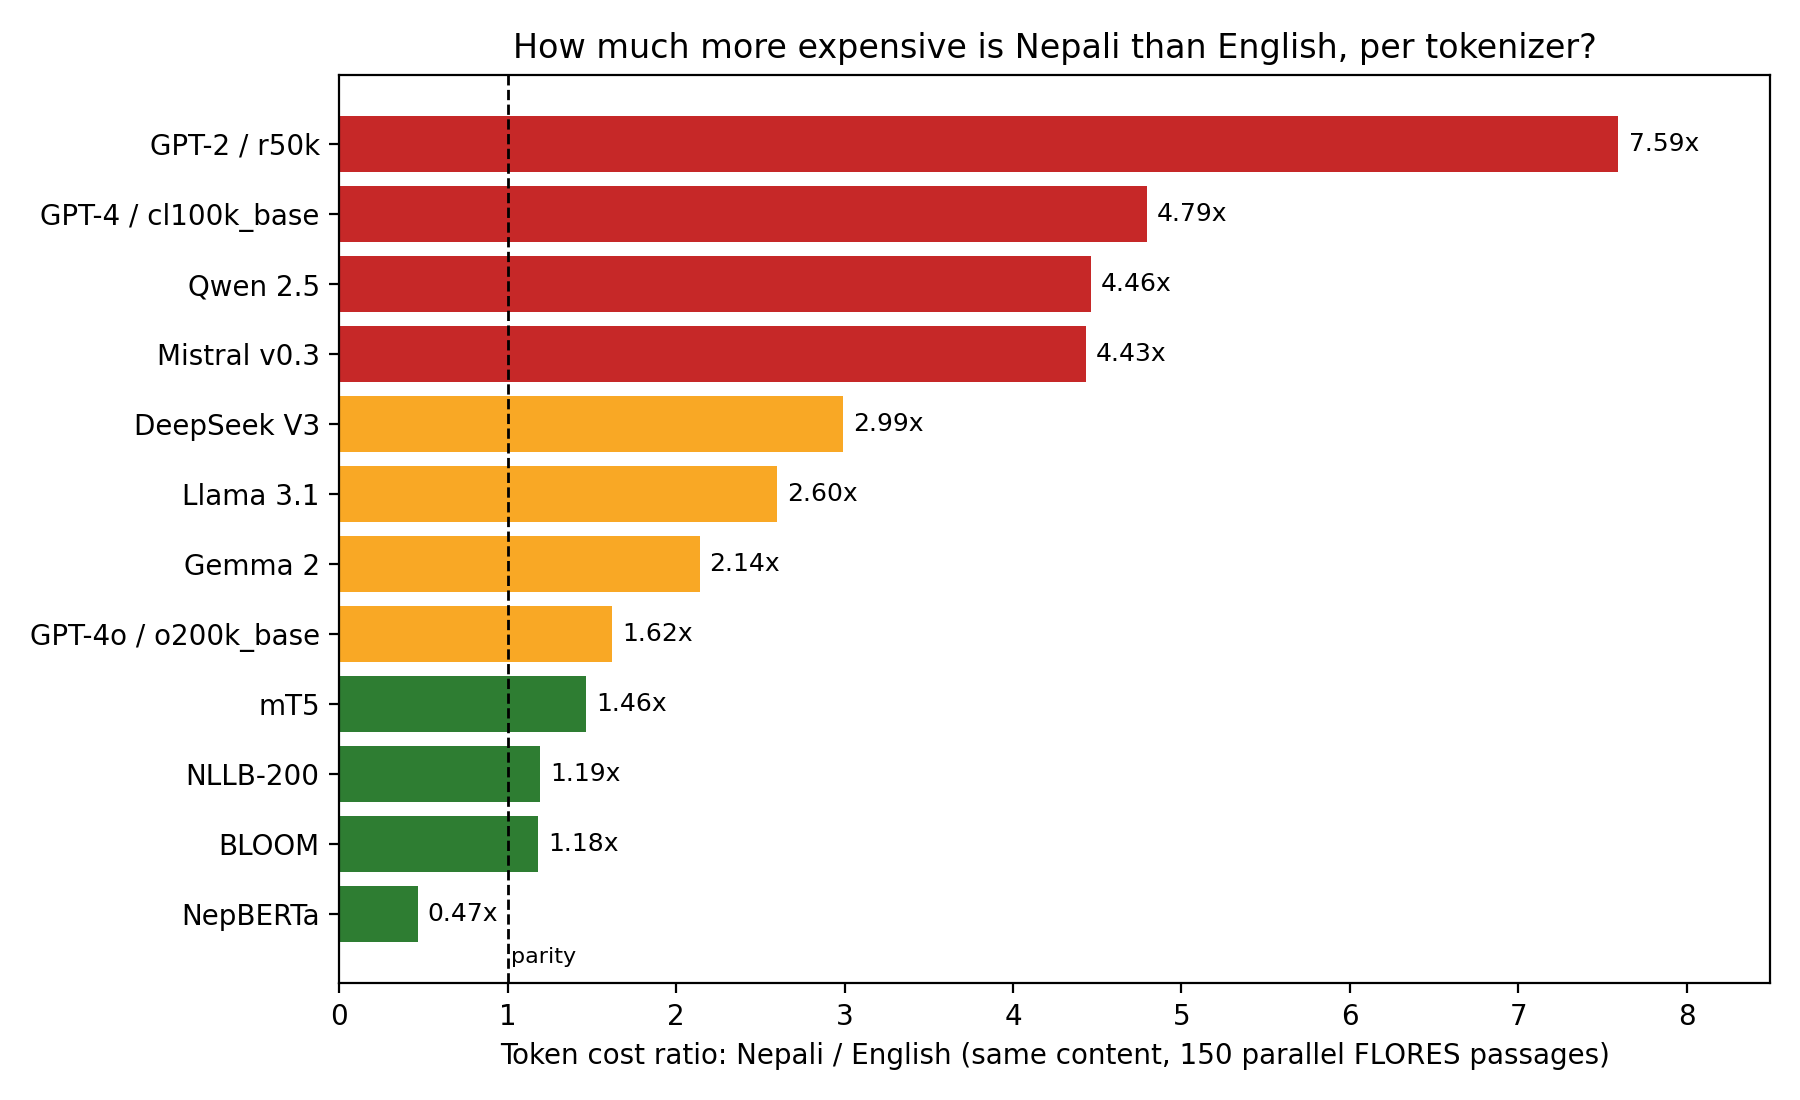
\includegraphics[width=\columnwidth]{figures/task1_cost_ratio.png}
\caption{Token cost ratio (Nepali/English) per tokenizer on identical parallel content. The dashed line marks parity.}
\label{fig:tok}
\end{figure}

\begin{figure}[t]
\centering
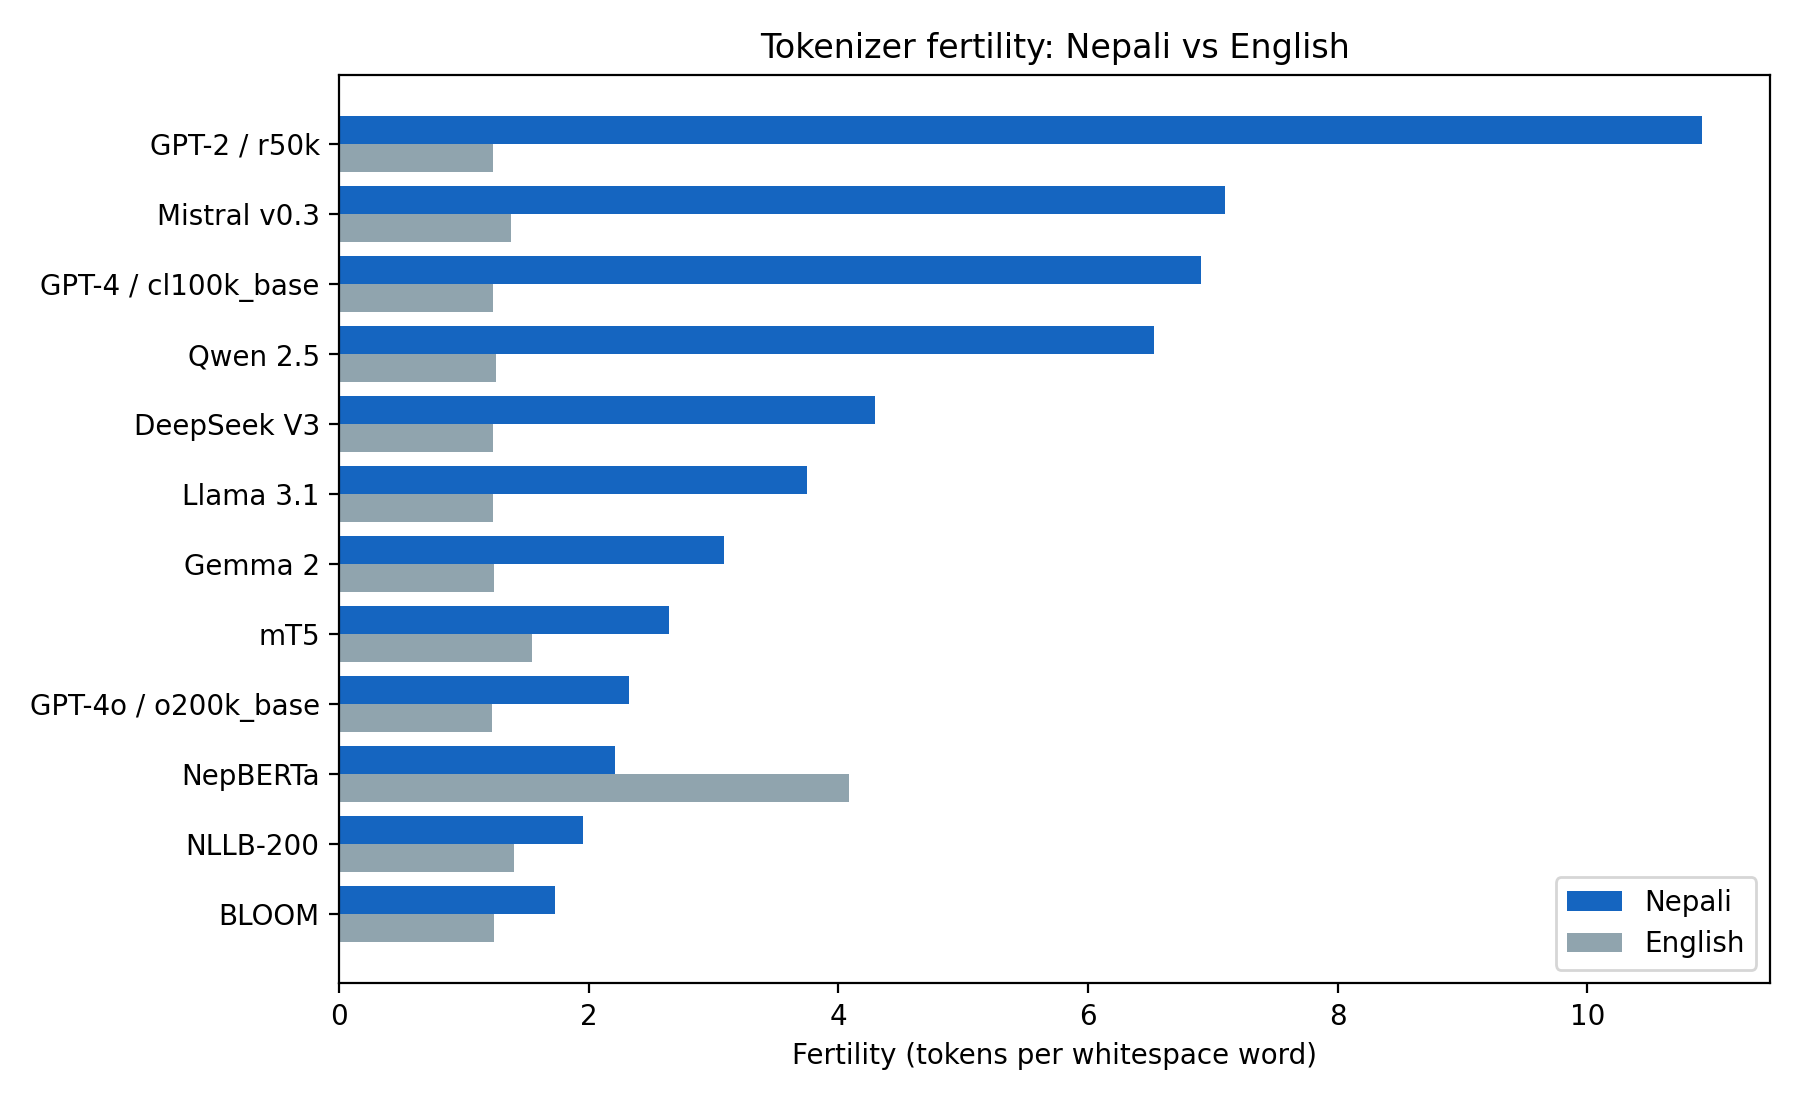
\includegraphics[width=\columnwidth]{figures/task1_fertility.png}
\caption{Tokenizer fertility (tokens per word) for Nepali and English. English fertility is nearly constant across tokenizers; Nepali fertility varies almost sixfold.}
\label{fig:fert}
\end{figure}

\subsection{Task 2: Reading Comprehension Under the Paired Design (RQ2)}
Table \ref{tab:qa} and Fig. \ref{fig:qa} report accuracy on items completed in both languages, so each row is a strictly controlled within-model comparison on identical content. Every model loses accuracy when the identical questions are asked in Nepali, and every gap except that of the small-sample local model is highly significant under McNemar's exact test.

The size of the loss orders cleanly by model class. Llama 3.1 8B drops 27.0 points, from 84.0\% to 57.0\%. Llama 4 Scout 17B and Llama 3.3 70B drop 10.0 and 10.1 points respectively; GPT-OSS 120B drops 8.5; and Gemini 3.1 Flash Lite drops 7.5, from 97.0\% to 89.5\%. The locally run Qwen2.5-0.5B, evaluated by log-likelihood on a 37-item paired subset, scores 46.0\% in English and 29.7\% in Nepali, the latter statistically indistinguishable from the 25\% chance floor: at this scale, Nepali comprehension has essentially not emerged at all.

The discordant-pair structure is strikingly one-sided and is reported per model in Table \ref{tab:qa}. For Gemini 3.1 Flash Lite, 15 items flipped from correct in English to wrong in Nepali and zero flipped the other way; for Llama 3.3 70B the counts are 18 versus 0; for Llama 3.1 8B, 57 versus 3. Language change is not adding noise symmetrically; it is removing capability directionally.

\begin{table}[t]
\caption{Paired reading comprehension (Belebele). Accuracy (\%) on items completed in both languages; b/c are discordant counts (correct in English only / correct in Nepali only); p from McNemar's exact test.}
\label{tab:qa}
\centering
\small
\begin{tabular}{lcccccc}
\toprule
Model & n & En & Ne & b & c & p \\
\midrule
Qwen2.5-0.5B (local) & 37 & 46.0 & 29.7 & 10 & 4 & 0.18 \\
Llama 3.1 8B & 200 & 84.0 & 57.0 & 57 & 3 & $6.3{\times}10^{-14}$ \\
Llama 4 Scout 17B & 200 & 96.0 & 86.0 & 22 & 2 & $3.6{\times}10^{-5}$ \\
Llama 3.3 70B & 178 & 97.2 & 87.1 & 18 & 0 & $7.6{\times}10^{-6}$ \\
GPT-OSS 120B & 200 & 95.0 & 86.5 & 20 & 3 & $4.9{\times}10^{-4}$ \\
Gemini 3.1 F.\ Lite & 200 & 97.0 & 89.5 & 15 & 0 & $6.1{\times}10^{-5}$ \\
\bottomrule
\end{tabular}
\end{table}

\begin{figure}[t]
\centering
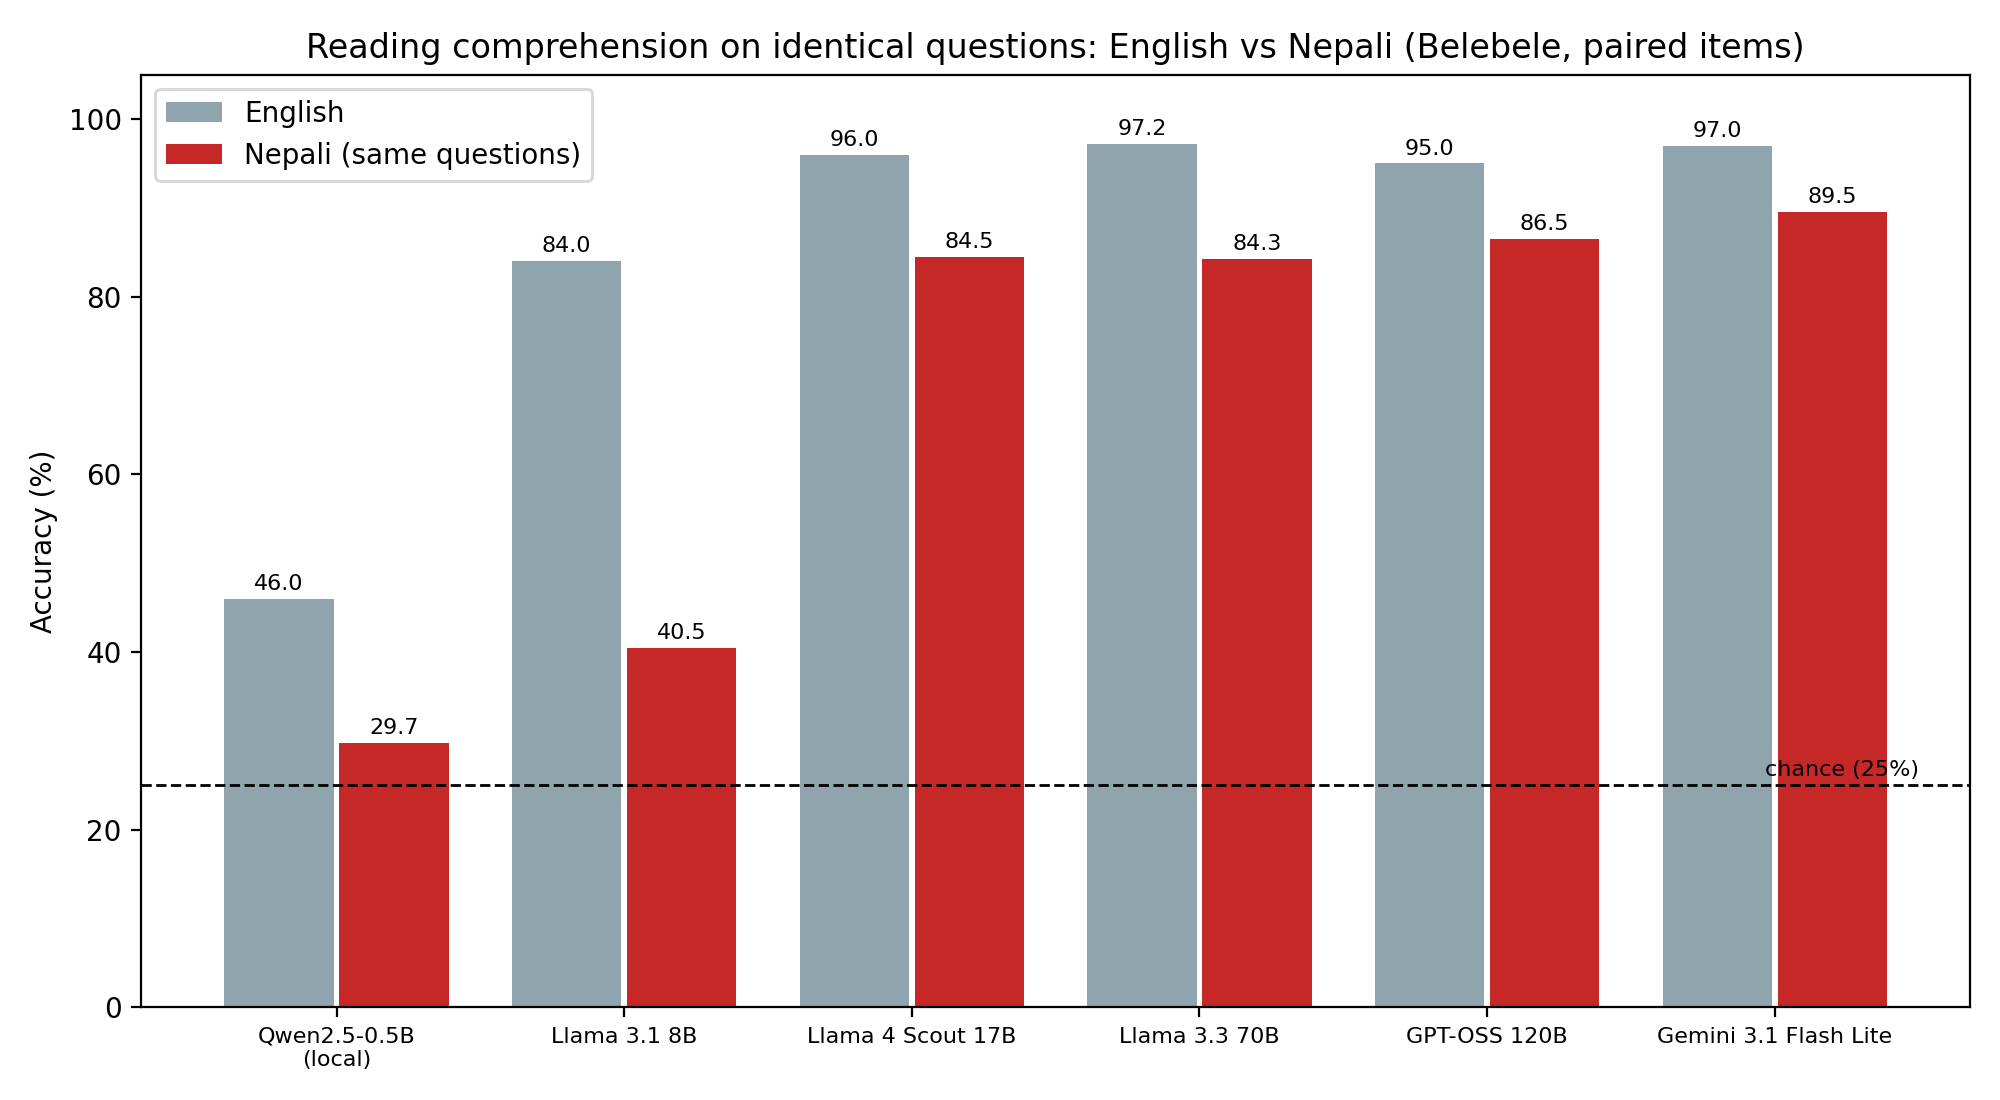
\includegraphics[width=\columnwidth]{figures/task2_qa_drop.png}
\caption{Reading comprehension accuracy on identical paired questions in English and Nepali. The dashed line marks the 25\% chance floor.}
\label{fig:qa}
\end{figure}

\subsection{A Methodological Finding: Devanagari Numeral Answers (RQ2, methodology)}
An initial scoring pass used a conventional answer parser that searched replies for the ASCII digits 1 to 4, the near-universal convention in multiple-choice evaluation code. Under that parser, Llama 3.1 8B appeared to abstain on 71 of 200 Nepali items and scored 40.5\%. Inspection of the published raw outputs revealed that these were not abstentions: the model was answering with Devanagari numerals (for example the character for 4 in Devanagari), that is, answering correctly formatted in the numeral system of the language it was addressed in. Re-parsing all stored raw replies with Devanagari digit support raised Llama 3.1 8B's Nepali accuracy from 40.5\% to 57.0\%, a 16.5-point correction, and also recovered 5 items for Llama 3.3 70B and 3 for Llama 4 Scout 17B. No English-language run was affected, and no reply in any run remained unparseable after the correction.

Both the initial error and its correction are preserved in the repository history. The episode is reported as a finding in its own right because its implications generalize: evaluation harnesses built with ASCII assumptions will systematically understate the ability of models that localize their output formatting, and will do so selectively for exactly the languages where accurate measurement matters most. Published multilingual leaderboard numbers produced by ASCII-only parsers should be treated with corresponding caution. It is also noteworthy that numeral localization behavior itself differs by model: Llama 3.1 8B localized numerals on 35.5\% of Nepali items, while GPT-OSS 120B and Gemini never did, an unmeasured dimension of output behavior that matters for downstream systems that parse model output.

\subsection{Task 3: Informal Native Nepali Is Much Harder than Formal Nepali (RQ3)}
Table \ref{tab:sent} and Fig. \ref{fig:sent} report sentiment results, including per-class F1. Although the same frontier models exceed 86\% on formal Belebele comprehension, none exceeds 67.1\% accuracy on three-class sentiment over informal native text (chance 33.3\%). GPT-OSS 120B leads at 67.1\% accuracy and 0.650 macro-F1; Llama 3.1 8B manages 51.9\%.

The per-class decomposition localizes the failure precisely: it is the neutral class. Llama 4 Scout 17B recalls 85.7\% of negative and 87.1\% of positive items but only 2.9\% of neutral ones (F1 = 0.055); Llama 3.1 8B recalls 10.0\% of neutral items; Gemini 3.1 Flash Lite, 15.6\%. Only GPT-OSS 120B achieves nontrivial neutral recall at 34.6\% (F1 = 0.481). The dominant error mode, visible in the published per-item outputs, is assigning emotional polarity to factual market commentary, for example labeling routine share-price observations as negative. Models appear to treat sentiment as a binary decision and force neutral content into it.

The 20 to 30 point gap between Belebele comprehension and native-register sentiment for the same models is one of the study's central observations: benchmarks built on formal translated text, including Belebele itself, substantially overstate practical capability on the language real users write, with its colloquial spelling, code-mixing, and domain slang.

\begin{table}[t]
\caption{Three-class sentiment on native Nepali social media text. Chance accuracy is 33.3\%. F1 columns are per-class. n varies where free-tier quotas ended runs early (Section IV-C).}
\label{tab:sent}
\centering
\small
\begin{tabular}{lcccccc}
\toprule
Model & n & Acc & mF1 & F1$_{neg}$ & F1$_{pos}$ & F1$_{neu}$ \\
\midrule
Llama 3.1 8B & 210 & 51.9 & .458 & .584 & .623 & .167 \\
Llama 4 Scout & 210 & 58.6 & .484 & .678 & .718 & .055 \\
Gemini 3.1 F.L. & 90 & 61.1 & .558 & .686 & .732 & .256 \\
GPT-OSS 120B & 158 & 67.1 & .650 & .695 & .773 & .481 \\
\bottomrule
\end{tabular}
\end{table}

\begin{figure}[t]
\centering
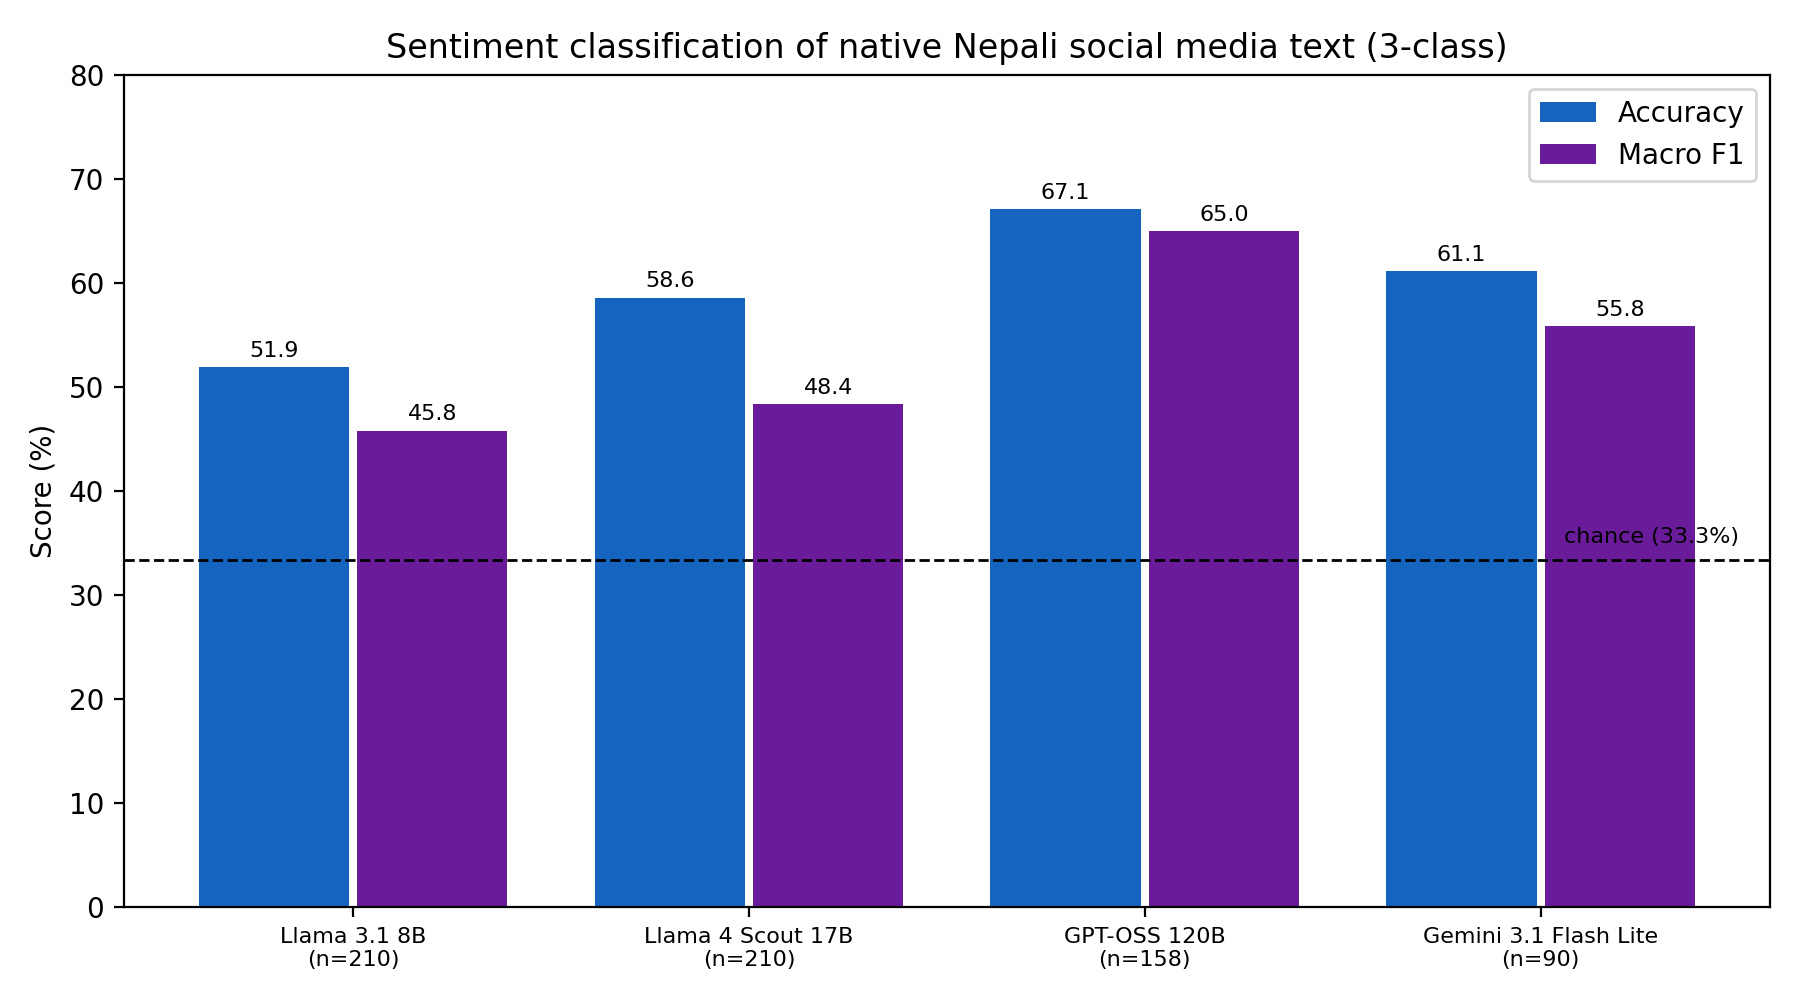
\includegraphics[width=\columnwidth]{figures/task3_sentiment.png}
\caption{Sentiment accuracy and macro-F1 on native informal Nepali text. The dashed line marks 33.3\% chance accuracy.}
\label{fig:sent}
\end{figure}

\subsection{Task 4: Models Read Nepali Better than They Write It (RQ4)}
Table \ref{tab:mt} reports translation quality for the two models whose runs completed within quota. Both are markedly better translating out of Nepali than into it. For Llama 3.1 8B the asymmetry is severe: 53.9 chrF++ from Nepali to English but 30.6 into Nepali, with BLEU collapsing from 28.9 to 7.7. Llama 4 Scout 17B shows the same direction of asymmetry at a uniformly higher level, 65.5 versus 49.1 chrF++. The 16.4-point directional gap for Scout and 23.3-point gap for the 8B model mirror the comprehension results: pretraining exposure to Nepali appears sufficient to support understanding well before it is sufficient to support fluent generation, consistent with generation requiring accurate modeling of the full output distribution while multiple-choice comprehension requires only relative ranking.

\begin{table}[t]
\caption{Passage-level translation quality on 150 parallel FLORES passages. chrF++ is primary; BLEU into Nepali uses flores200 sentencepiece tokenization.}
\label{tab:mt}
\centering
\small
\begin{tabular}{lcccc}
\toprule
 & \multicolumn{2}{c}{ne $\rightarrow$ en} & \multicolumn{2}{c}{en $\rightarrow$ ne} \\
Model & chrF++ & BLEU & chrF++ & BLEU \\
\midrule
Llama 3.1 8B & 53.9 & 28.9 & 30.6 & 7.7 \\
Llama 4 Scout 17B & 65.5 & 40.5 & 49.1 & 27.3 \\
\bottomrule
\end{tabular}
\end{table}

\subsection{Task 5: Nepali RAG Is Feasible Today, with the Right Embeddings (RQ5)}
Table \ref{tab:ret} and Fig. \ref{fig:ret} report retrieval quality. BGE-M3 leads with 84.0\% Recall@1 and 0.879 MRR@10 monolingually, with 95.0\% of gold passages inside the top 10; the multilingual E5 models follow at 77.0 to 77.5\% Recall@1. These are strong absolute numbers over a 488-document corpus and indicate that the retrieval stage of a Nepali RAG system is a solved problem at this scale with current open models.

Two failure patterns matter for practitioners. First, the English-only control retrieves essentially nothing: 1.0\% Recall@1 monolingually. Default English embedding stacks pointed at Devanagari content do not degrade gracefully; they fail outright. Second, paraphrase-multilingual-MiniLM, a model widely deployed for multilingual applications, scores only 15.0\% monolingually while reaching 52.5\% cross-lingually with English queries. The asymmetry is diagnostic: its cross-lingual alignment is functional but its underlying Nepali text representation is weak, so its multilingual label conceals a large per-language capability gap.

Third, and most useful architecturally: for the strongest models, cross-lingual retrieval with English queries performs on par with monolingual retrieval (BGE-M3: 81.0\% versus 84.0\%; e5-small: 79.0\% versus 77.5\%). Systems can therefore accept English queries over Nepali document collections, or mix query languages, without a dedicated translation step.

\begin{table}[t]
\caption{Retrieval over a 488-passage Nepali corpus, 200 queries. Mono: Nepali queries; Cross: English queries. R@k in \%.}
\label{tab:ret}
\centering
\small
\begin{tabular}{lcccccc}
\toprule
 & \multicolumn{3}{c}{Mono} & \multicolumn{3}{c}{Cross} \\
Model & R@1 & R@10 & MRR & R@1 & R@10 & MRR \\
\midrule
BGE-M3 & 84.0 & 95.0 & .879 & 81.0 & 96.0 & .863 \\
m-e5-small & 77.5 & 94.0 & .829 & 79.0 & 97.0 & .855 \\
m-e5-base & 77.0 & 92.0 & .817 & 76.5 & 96.5 & .829 \\
LaBSE & 58.0 & 82.0 & .659 & 63.5 & 85.5 & .717 \\
p-m-MiniLM & 15.0 & 37.0 & .212 & 52.5 & 81.0 & .619 \\
MiniLM-L6 (ctrl) & 1.0 & 3.0 & .013 & 4.5 & 9.0 & .053 \\
\bottomrule
\end{tabular}
\end{table}

\begin{figure}[t]
\centering
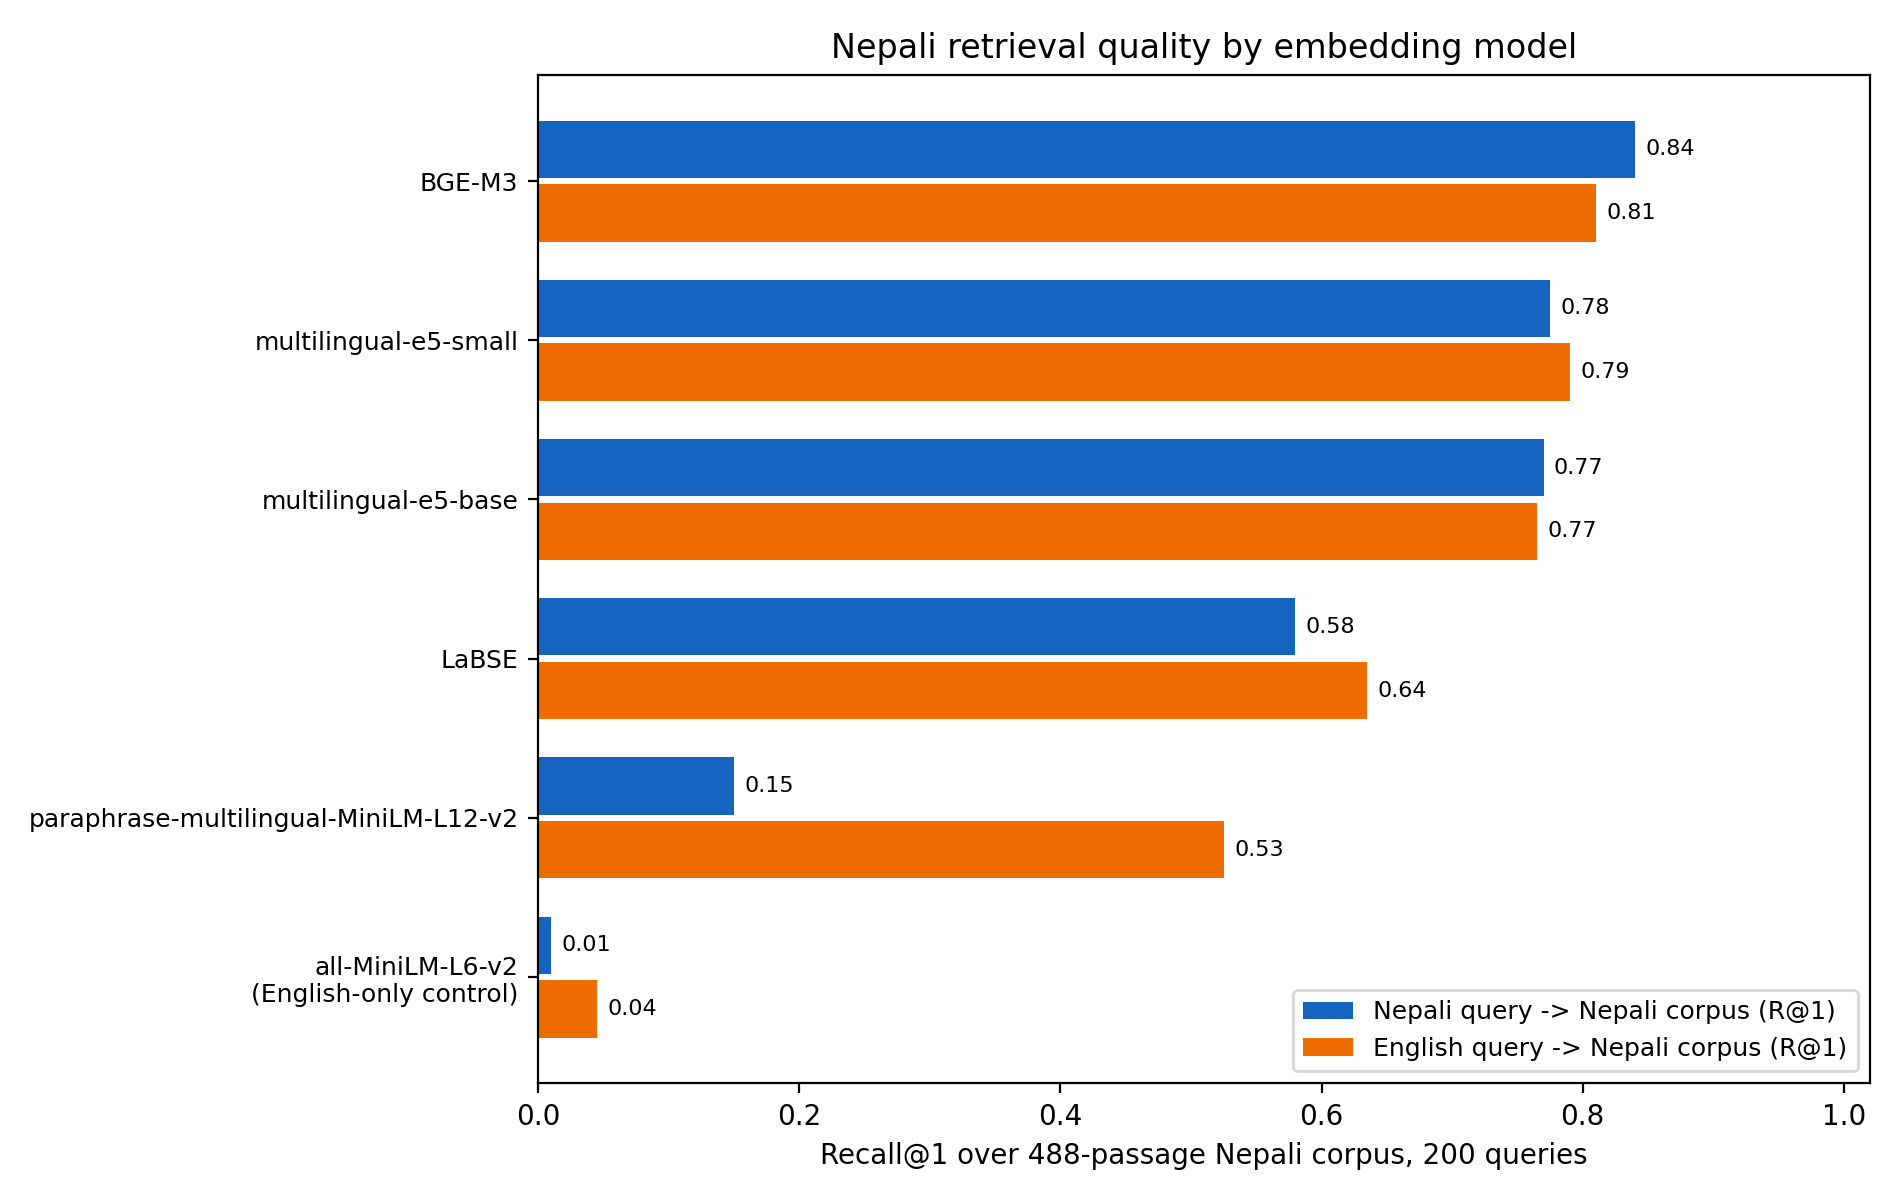
\includegraphics[width=\columnwidth]{figures/task5_retrieval_r1.png}
\caption{Recall@1 by embedding model, monolingual and cross-lingual settings, including the English-only negative control.}
\label{fig:ret}
\end{figure}

\section{Discussion}
\subsection{The Nepali Tax Is Real and Layered}
Combining the tasks yields a composite picture of what a Nepali speaker experiences today. Interacting with a cl100k-era commercial system, they pay a monetary surcharge of up to 4.8x per unit of content (Task 1), receive a context window effectively 4.8x smaller, wait longer per response since decoding cost scales with sequence length, and on top of these obtain measurably worse answers (Tasks 2 to 4). These penalties compound: the same rupee buys fewer tokens, each token carries less meaning, and the meaning is understood less reliably. The tokenizer component, however, is demonstrably fixable. The threefold improvement from cl100k to o200k within one product generation, and the near-parity of NLLB-200 and BLOOM, establish that a vocabulary respecting Devanagari is an engineering decision that vendors can simply make.

\subsection{Scale and Recency Close the Comprehension Gap but Not the Production Gap}
The paired design isolates language as the only variable, and the ordering is unambiguous: the English-to-Nepali comprehension drop shrinks from 27.0 points at 8B scale to 7.5 points for the frontier commercial model, with all gaps significant and all discordance one-directional. Two further patterns qualify the optimism. First, generation into Nepali lags comprehension of Nepali across the board (Task 4), so systems that must write Nepali, such as government service chatbots or educational tools, face a harder problem than systems that must only read it. Second, the informal register remains difficult even for the strongest models tested (Task 3), and real users write in the informal register. A model selection decision based on Belebele-style scores alone would materially overestimate deployed quality.

\subsection{Evaluation Infrastructure Is Itself Biased Toward English}
The Devanagari numeral episode (Section V-C) deserves emphasis beyond its 16.5-point local effect. The error was not in the model, which behaved reasonably by localizing its output; it was in evaluation tooling that encoded an ASCII worldview. Such tooling is shared, copied, and rarely audited per language. If a single-language deep dive with published raw outputs surfaced this within one benchmark, aggregate multilingual leaderboards computed by the same class of parser plausibly contain similar distortions for other numeral systems (Arabic-Indic, Bengali, Burmese, and others). Publishing raw per-item outputs, as done here, is what made the error discoverable and correctable; the practice is recommended as a norm for multilingual evaluation.

\subsection{Practical Guidance for Builders}
For teams building Nepali-facing systems today, the results support concrete recommendations. For retrieval: use BGE-M3 or multilingual E5; never English-only defaults, which fail completely rather than degrade; English queries over Nepali corpora are viable with these models, removing the need for query translation. For generation: assume open models of 8B and below are unreliable in Nepali until verified on native-register data; model families differ far more in Nepali than their English leaderboard positions suggest, so per-language evaluation before selection is not optional. For cost planning: tokenizer choice changes Nepali serving costs by a factor of four between vendors at equal per-token price, so price comparisons must be made in tokens-per-Nepali-document, not tokens. For output handling: parse numerals and labels in the script of the interaction language.

\subsection{Zero-Budget Reproducibility as a Template}
Every number in this paper was produced on one CPU core plus free API tiers, with quota-truncated sample sizes disclosed rather than hidden, and with the full audit trail published. This is offered deliberately as a template. The researchers best positioned to evaluate low-resource languages, native speakers embedded in the linguistic community, are often the least resourced financially. The methodology here, frozen open data, resumable evaluation with published raw outputs, paired designs with exact tests, and free inference tiers, is transferable as-is to Sinhala, Khmer, Amharic, or any of the hundreds of languages in the same position as Nepali.

\section{Limitations}
Several limitations bound the conclusions. Sample sizes are modest (150 to 210 items per task), reflecting the zero-budget constraint; confidence in individual point estimates is correspondingly limited, though the paired design and exact tests make the central language-gap findings robust. Several API runs are quota-truncated prefix samples, with n as low as 90 for one sentiment run; affected sample sizes are stated wherever results appear, and truncation is by fixed item order, not selection. Translation is evaluated at passage level rather than sentence level because sentence-aligned open Nepali test sets are gated; passage-level chrF++ remains meaningful but is not directly comparable to sentence-level literature numbers. A single prompt template per task and language is used at temperature 0, so prompt sensitivity is unmeasured; results characterize default behavior, not attainable ceilings. Belebele passages are public data and partial training contamination cannot be excluded; contamination would, however, compress rather than create the observed language gaps, since both language versions are equally public. The sentiment corpus inherits undocumented upstream annotation methodology; label semantics were verified by native speaker inspection and a validation sample ships with the repository, but original annotation noise is inherited, and the corpus is domain-skewed toward financial and video commentary. Closed models without free tiers (GPT-4o, Claude) could not be included, and the Gemini flagship free quota permitted only an excluded 21-item probe. Retrieval uses questions as queries over the passages they were written against, a favorable setting relative to open-web retrieval. Finally, all findings concern one language; the methodology transfers, but the numbers should not be assumed to.

\section{Future Work}
Natural extensions include: sentence-level translation evaluation once open aligned Nepali test sets become available; a native-register comprehension set to complement Belebele's formal register, constructed with native speaker annotation; inclusion of paid frontier models and Nepali-focused fine-tunes as budget permits; prompt-sensitivity and few-shot analyses; extension of the numeral-parsing audit to other Brahmic-script languages; and periodic re-runs of the frozen suite as new model generations appear, for which the repository is structured to serve as a longitudinal record.

\section{Conclusion}
This paper introduced a reproducible, openly licensed, zero-budget benchmark of Nepali capability spanning cost, comprehension, real-register understanding, generation, and retrieval, evaluated across six language models, six embedding models, and twelve tokenizers, with paired statistical testing and fully published raw outputs. The findings are direct. Current AI systems charge Nepali speakers up to 4.8 times more per unit of meaning, a penalty that is a tokenizer design choice rather than a property of the script. They understand Nepali measurably worse than English on identical content, with the gap shrinking from 27.0 points to 7.5 points as models grow in scale and recency, and every gap statistically significant and directionally one-sided. They read Nepali substantially better than they write it, and they handle the formal Nepali of benchmarks far better than the informal Nepali of real users, failing almost completely on neutral-class judgments of native text. Evaluation tooling itself carries English assumptions: a standard ASCII answer parser understated one model's Nepali accuracy by 16.5 points because the model, reasonably, answered in Devanagari numerals. And yet the infrastructure for Nepali applications is closer than the generation results suggest: off-the-shelf multilingual embeddings already retrieve Nepali passages with 84\% top-1 accuracy, monolingually and cross-lingually alike. Both the cost gap and the comprehension gap are demonstrably closable, and the benchmark is released in full so that progress against them can be measured rather than asserted.

\section*{Data and Code Availability}
All code, frozen evaluation data, provenance documentation, raw per-item model outputs, statistical analyses, and figure generation scripts are available at \url{https://github.com/RameshKadariya/nepali-llm-benchmark} under the MIT license, with Belebele-derived data remaining CC-BY-SA 4.0. The repository history preserves the full evaluation timeline, including the scoring correction described in Section V-C.

\section*{Acknowledgment}
The author thanks the maintainers of the open datasets and open-weight models that made a zero-budget study possible, and the providers of free inference tiers used under their published terms.

\appendix
\section{Prompt Templates}
All evaluation prompts, verbatim as used, in both languages, are stored in the repository source files (\texttt{src/task2\_qa\_api.py}, \texttt{src/task3\_sentiment\_api.py}, \texttt{src/task4\_translation\_api.py}). The English comprehension template is reproduced here; the Nepali template is its direct translation with instructions in Nepali:

\begin{quote}\small
Read the passage below and choose the correct answer to the question. Reply with only the number of the correct option (1, 2, 3 or 4).

Passage: \{passage\}

Question: \{question\}

Options:\\
1. \{option 1\}\\
2. \{option 2\}\\
3. \{option 3\}\\
4. \{option 4\}

Answer:
\end{quote}

The translation template instructs: ``Translate the following Nepali text to English. Output only the English translation, nothing else.'' (and symmetrically for the reverse direction). The sentiment template is written in Nepali and requests exactly one word from the three Nepali label words.

\begin{thebibliography}{00}
\bibitem{bandarkar2024belebele} L. Bandarkar et al., ``The Belebele benchmark: a parallel reading comprehension dataset in 122 language variants,'' in \emph{Proc. 62nd Annu. Meeting Assoc. Comput. Linguistics (ACL)}, 2024.
\bibitem{goyal2022flores} N. Goyal et al., ``The FLORES-101 evaluation benchmark for low-resource and multilingual machine translation,'' \emph{Trans. Assoc. Comput. Linguistics}, vol. 10, pp. 522--538, 2022.
\bibitem{nllb2022} NLLB Team et al., ``No language left behind: scaling human-centered machine translation,'' arXiv:2207.04672, 2022.
\bibitem{petrov2023tokenizers} A. Petrov, E. La Malfa, P. H. S. Torr, and A. Bibi, ``Language model tokenizers introduce unfairness between languages,'' in \emph{Adv. Neural Inf. Process. Syst. (NeurIPS)}, 2023.
\bibitem{ahia2023cost} O. Ahia et al., ``Do all languages cost the same? Tokenization in the era of commercial language models,'' in \emph{Proc. EMNLP}, 2023.
\bibitem{wang2024e5} L. Wang et al., ``Multilingual E5 text embeddings: a technical report,'' arXiv:2402.05672, 2024.
\bibitem{chen2024bgem3} J. Chen, S. Xiao, P. Zhang, K. Luo, D. Lian, and Z. Liu, ``BGE M3-Embedding: multi-lingual, multi-functionality, multi-granularity text embeddings through self-knowledge distillation,'' arXiv:2402.03216, 2024.
\bibitem{feng2022labse} F. Feng, Y. Yang, D. Cer, N. Arivazhagan, and W. Wang, ``Language-agnostic BERT sentence embedding,'' in \emph{Proc. 60th Annu. Meeting Assoc. Comput. Linguistics (ACL)}, 2022.
\bibitem{reimers2019sbert} N. Reimers and I. Gurevych, ``Sentence-BERT: sentence embeddings using Siamese BERT-networks,'' in \emph{Proc. EMNLP-IJCNLP}, 2019.
\bibitem{timilsina2022nepberta} S. Timilsina, M. Gautam, and B. Bhattarai, ``NepBERTa: Nepali language model trained in a large corpus,'' in \emph{Proc. 2nd Conf. Asia-Pacific Chapter Assoc. Comput. Linguistics (AACL-IJCNLP)}, 2022.
\bibitem{popovic2017chrf} M. Popovi\'c, ``chrF++: words helping character n-grams,'' in \emph{Proc. 2nd Conf. Machine Translation (WMT)}, 2017.
\bibitem{papineni2002bleu} K. Papineni, S. Roukos, T. Ward, and W.-J. Zhu, ``BLEU: a method for automatic evaluation of machine translation,'' in \emph{Proc. 40th Annu. Meeting Assoc. Comput. Linguistics (ACL)}, 2002.
\bibitem{post2018sacrebleu} M. Post, ``A call for clarity in reporting BLEU scores,'' in \emph{Proc. 3rd Conf. Machine Translation (WMT)}, 2018.
\bibitem{grattafiori2024llama} A. Grattafiori et al., ``The Llama 3 herd of models,'' arXiv:2407.21783, 2024.
\bibitem{qwen2025} Qwen Team, ``Qwen2.5 technical report,'' arXiv:2412.15115, 2024.
\bibitem{openai2025gptoss} OpenAI, ``gpt-oss-120b and gpt-oss-20b model card,'' arXiv:2508.10925, 2025.
\bibitem{mcnemar1947} Q. McNemar, ``Note on the sampling error of the difference between correlated proportions or percentages,'' \emph{Psychometrika}, vol. 12, no. 2, pp. 153--157, 1947.
\end{thebibliography}

\balance
\end{document}
